%%% The ``\documentclass'' command has one parameter, based on the kind of
%%% document you are preparing.
%%%
%%% [annual] - Technical paper accepted for presentation at the ACM SIGGRAPH 
%%%   or SIGGRAPH Asia annual conference.
%%% [sponsored] - Short or full-length technical paper accepted for 
%%%   presentation at an event sponsored by ACM SIGGRAPH
%%%   (but not the annual conference Technical Papers program).
%%% [abstract] - A one-page abstract of your accepted content
%%%   (Technical Sketches, Posters, Emerging Technologies, etc.). 
%%%   Content greater than one page in length should use the "[sponsored]"
%%%   parameter.
%%% [preprint] - A preprint version of your final content.
%%% [review] - A technical paper submitted for review. Includes line
%%%   numbers and anonymization of author and affiliation information.

\documentclass[annual]{acmsiggraph}

\usepackage{par06}
\usepackage{amsmath}
\usepackage{amssymb}
\usepackage{amsthm}
\usepackage{overpic}
\usepackage{contour}\contourlength{1pt}
\usepackage{color}

\long\def\nix#1{\relax}


\def\div{\DID YOU RELLY WANT TO USE \div?}
\def\<{\mathchoice{\big\langle}{\langle}{\langle}{\langle}}
\def\>{\mathchoice{\big\rangle}{\rangle}{\rangle}{\rangle}}
%\def\lll{\mathopen{\mbox{$\<\hskip-.5ex\<$}}}
%\def\rrr{\mathclose{\mbox{$\>\hskip-.5ex\>$}}}
\def\wh{\widehat}
%\def\II{\mbox{I\hskip-0.1exI}}
%\def\pu{{\partial\over\partial u}}
%\def\du{{d\over d u}}
%\def\hinauf#1#2{{\mathop{#1}\limits^{\vbox to-.32564ex{\kern-.4652ex
%   \hbox{\normalfont #2}\vss}}}}
%\def\dddot#1{\hinauf{#1}{...}}
%\def\ddddot#1{\hinauf{#1}{....}}
%\def\str{/\penalty10000\hskip0pt}
%\def\d#1dot#2{\dddddot{#2}}
\newtheorem{theorem}{Theorem}
\newtheorem{prop}[theorem]{Proposition}
\def\Div{\mathop{\textrm{div}}\nolimits}
\def\tr{\mathop{\textrm{tr}}\nolimits}
\def\rel{{\mathord{\text{\rm rel}}}}
\def\const{{\mathord{\textrm{const}}}}
\def\ess{s}
\def\Hess#1{{\def\testess{#1}\nabla^2\ifx\testess\ess\!s\else #1\fi}}
\def\Hess#1{\text{$\nabla^2\hskip-.2ex #1$}}
\def\Forcevector{\Big(\mbox{\scriptsize
	\def\arraystretch{0.8}\begin{tabular}{@{\,}c@{\,}}
	0 \\ 0 \\ $A_i F_i$
	\end{tabular}}\Big)}

\def\lput(#1,#2)#3{\put(#1,#2){\hbox to 0pt{\hss{#3}}}}
\def\cput(#1,#2)#3{\put(#1,#2){\hbox to 0pt{\hss{#3}\hss}}}
\definecolor{blau}{rgb}{0.15,0.2,0.3}
%\definecolor{rot}{rgb}{0.7,0.5,0.2}
\definecolor{drot}{rgb}{0.7,0,0.1}
\definecolor{grey}{rgb}{0.6,0.6,0.6}
\definecolor{lightgrey}{rgb}{0.8,0.8,0.8}
\definecolor{gelb}{rgb}{.55,.40,.1}


\outer\def\proclaim #1. #2\par{\noindent{\bf#1.\enspace}{\it#2\par}}


%\usepackage{mathrsfs}
\def\SS{{\mathcal S}}
\def\RR{{\mathcal R}}


\newcommand{\todo}[1]{\textcolor{red}{#1}}
\newcommand{\secref}[1]{(\S\ref{#1})}

%%% If you are submitting your paper to one of our annual conferences - the 
%%% ACM SIGGRAPH conference held in North America, or the SIGGRAPH Asia 
%%% conference held in Southeast Asia - there are several commands you should 
%%% consider using in the preparation of your document.

%%% 1. ``\TOGonlineID''
%%% When you submit your paper for review, please use the ``\TOGonlineID''
%%% command to include the online ID value assigned to your paper by the
%%% submission management system. Replace '45678' with the value you were
%%% assigned.

\TOGonlineid{0043}

%%% 2. ``\TOGvolume'' and ``\TOGnumber''
%%% If you are preparing a preprint of your accepted paper, and your paper
%%% will be published in an issue of the ACM ``Transactions on Graphics''
%%% journal, replace the ``0'' values in the commands below with the correct
%%% volume and number values for that issue - you'll get them before your
%%% final paper is due.

\TOGvolume{0}
\TOGnumber{0}

%%% 3. ``TOGarticleDOI''
%%% The ``TOGarticleDOI'' command accepts the DOI information provided to you
%%% during production, and which makes up the URLs which identifies the ACM
%%% article page and direct PDF link in the ACM Digital Library.
%%% Replace ``1111111.2222222'' with the values you are given.

\TOGarticleDOI{1111111.2222222}

%%% 4. ``\TOGprojectURL'', ``\TOGvideoURL'', ``\TOGdataURL'', ``\TOGcodeURL''
%%% If you would like to include links to personal repositories for auxiliary
%%% material related your research contribution, you may use one or more of
%%% these commands to define an appropriate URL. The ``\TOGlinkslist'' command
%%% found just before the first section of your document will add hyperlinked
%%% icons to your document, in addition to hyperlinked icons which point to
%%% the ACM Digital Library article page and the ACM Digital Library-held PDF.

\TOGprojectURL{}
\TOGvideoURL{}
\TOGdataURL{}
\TOGcodeURL{}

%%% Replace ``PAPER TEMPLATE TITLE'' with the title of your paper or abstract.

\title{Design of Self-supporting Surfaces}

%%% The ``\author{}'' command takes the names and affiliations of each of the
%%% authors of your paper or abstract. The ``\thanks{}'' command takes the
%%% contact information for each author.
%%% For multiple authors, separate each author's information by the ``\and''
%%% command.

%\author{Roy G. Biv\thanks{e-mail: roy.g.biv@aol.com}\\ Starbucks Research %
%\and Ed Grimley\thanks{e-mail:ed.grimley@aol.com}\\Nigel Mansell\thanks{nigelf1@msn.com}\\ Grimley Widgets, Inc. %
%\and Martha Stewart\thanks{e-mail:martha.stewart@marthastewart.com}\\ Martha Stewart Enterprises \\ Microsoft Research}

%%% The ``pdfauthor'' command accepts the authors of the work,
%%% comma-delimited, and adds this information to the PDF metadata.

\pdfauthor{Anonymous}

%%% Keywords that describe your work. The ``\keywordlist'' command will print
%%% them out.

\keywords{TODO}

%%% The ``\begin{document}'' command is the start of the document.

%%% If you have user-defined macros, you may include them here.

% example of a user-defined macro called ``remark.''
% \newcommand{\remark}[1]{\textcolor{red}{#1}}

\begin{document}

%%% A ``teaser'' image appears under the title and affiliation information,
%%% horizontally centered, and above the two columns of text. This is OPTIONAL.
%%% If you choose to have a ``teaser'' image, it needs to be placed between
%%% ``\begin{document}'' and ``\maketitle.''

%\teaser{
%   \includegraphics[height=1.5in]{images/sampleteaser}
%   \caption{Spring Training 2009, Peoria, AZ.}
%}

%%% The ``\maketitle'' command must appear after ``\begin{document}'' and,
%%% if you have one, after the definition of your ``teaser'' image, and
%%% before the first ``\section'' command.

\maketitle

%%% Your paper's abstract goes in its own section.

\begin{abstract}

\todo{TODO}

\vspace*{6cm}

\end{abstract}

%%% ACM Computing Review (CR) categories.
%%% See <http://www.acm.org/class/1998/> for details.
%%% The ``\CRcat'' command takes four arguments.

\begin{CRcatlist}
  \CRcat{I.3.5}{Computer Graphics}{Computational Geometry and Object Modeling}{Curve, surface, solid, and object representations};
\end{CRcatlist}

%%% The ``\keywordlist'' command prints out the keywords.

\keywordlist

%%% The ``\TOGlinkslist'' command will insert hyperlinked icon(s) to your
%%% paper. This includes, at a minimum, hyperlinked icons to the ACM article
%%% page and the ACM Digital Library-held PDF. If you added URLs to
%%% ``\TOGprojectURL'' or the other, similar commands, they will be added to
%%% the list of icons.
%%% Note: this functionality only works for annual-conference papers.

\TOGlinkslist

%%% The ``\copyrightspace'' command 
%%% Do not remove this command.

\copyrightspace

%%% This is the first section of the body of your paper.

\section{Introduction}

\todo{TODO gentle introduction to self-supporting surfaces, assumptions about the model, importance to architecture etc}


Vaulted masonry structures are among the simplest and at the same time 
most elegant solutions for creating curved shapes in building 
construction. This is the reason why they have been an object of interest 
since antiquity, and why they continue to be an active topic of research 
in today's engineering community. The shapes range from convex to 
non-convex to freeform (see Figures \ref{fig:tholos} and \ref{fig:block}).

Our paper is concerned with a combined geometry+statics analysis of {\em 
self\dash supporting} masonry and with tools for the interactive modeling 
of freeform self\dash supporting structures. Here `self\dash supporting' 
means that the structure, considered as an arrangement of blocks (bricks, 
stones), holds together by itself, and additional support, additional 
chains and similar are present only during construction. Our analysis is 
based on the following assumptions, which follow the classic 
\cite{Heyman66}:


{\it Assumption 1:} Masonry has no tensile strength, but the individual 
building blocks do not slip against each other (because of friction or 
mortar). On the other hand, their compressive strength is sufficiently 
high so that failure of the structure is by a sudden change in geometry, 
such as shown by Figure \ref{fig:block}, and not by material failure.

{\it Assumption 2 (the Safe Theorem)}: If a system of forces can be found 
which is in equilibrium with the load on the structure and which is 
contained within the masonry envelope then the structure will carry the 
loads, although the actually occurring forces may not be those postulated.

Our approach is twofold: We first investigate the continuous case of a 
smooth surface under stress which turns out to be governed by the so\dash 
called {\em Airy stress function}. This mathematical model is called a 
{\em membrane} in the engineering literature and has been applied to the 
analysis of masonry before. The surface is self\dash supporting if and 
only if stresses are entirely compressive (i.e., the Airy function is 
convex).

For computational purposes, stresses are discretized as a fictitious {\em 
thrust network} contained in the masonry structure. This is a system of 
forces which together with the structure's deadload is in equilibrium. It 
can be interpreted as a finite element discretization of continuous case, 
and it turns out to have very interesting geometry: we have a polyhedral 
Airy stress function and a reciprocal force diagram, both of which are 
present in earlier work. Our own contributions are the following:



	\begin{figure}[t]
	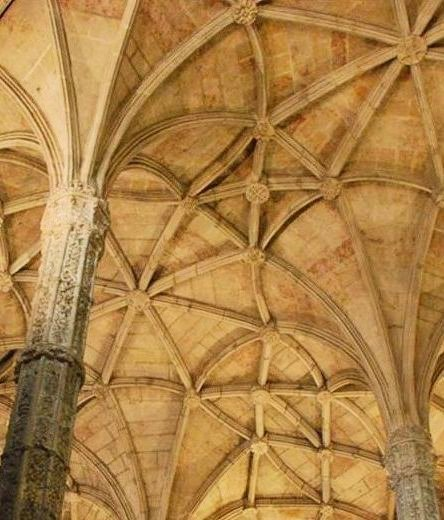
\includegraphics[height=.35\columnwidth]{fotos/gothicvaults1}\hfill
	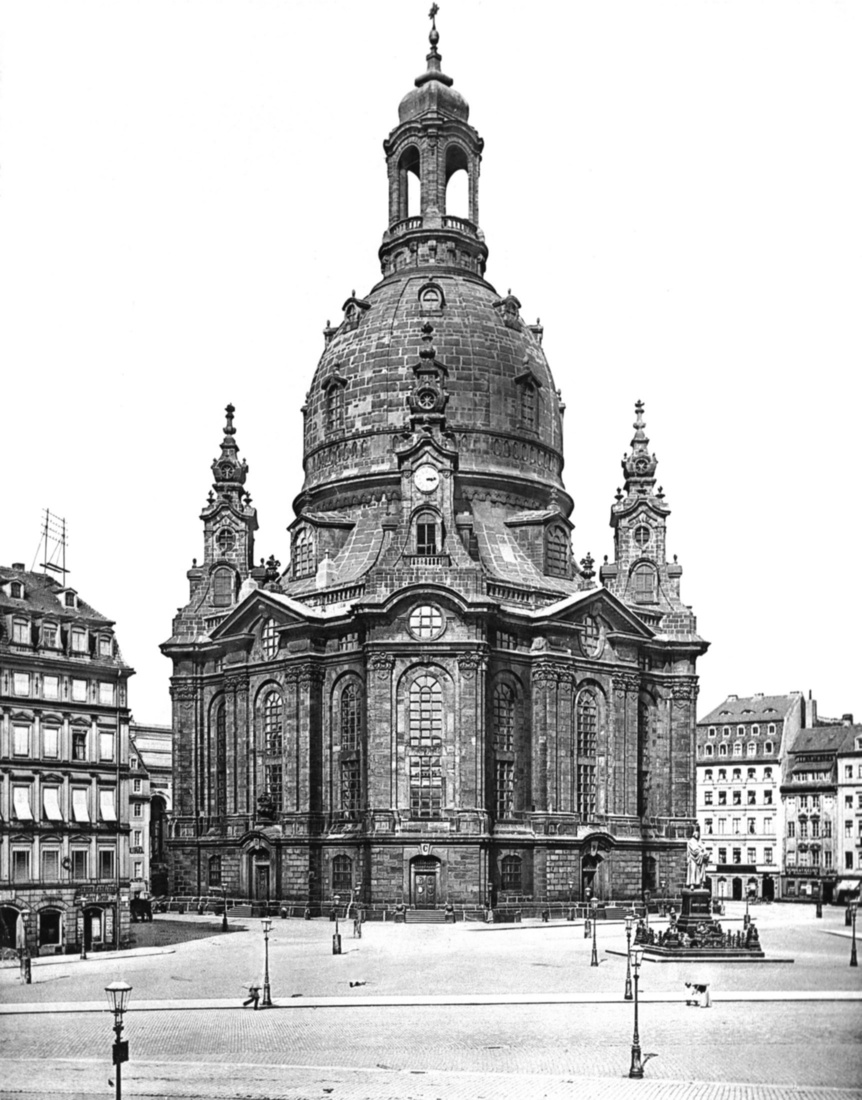
\includegraphics[height=.35\columnwidth]{fotos/Frauenkirche_um_1897}
	\hfill
	\hfill
	\begin{minipage}[b]{.37\columnwidth} \caption{Nonconvex self\dash 
supporting masonry. Left: vaults of a gothic cathedral; Right: dome of 
Frauenkirche, Dres\-den}
	\label{fig:tholos}
	\end{minipage}
	\bigskip


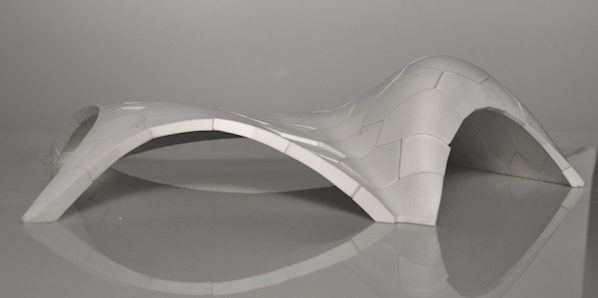
\includegraphics[height=.245\columnwidth]{fotos/project_24_77.png}\hfill
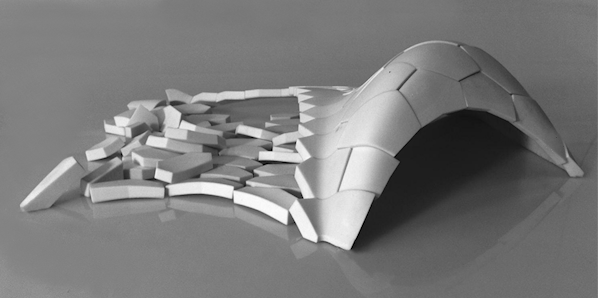
\includegraphics[height=.245\columnwidth]{fotos/project_24_81.png}
	\caption{Freeform masonry vault (left) and failure of the same 
(right). These are mock\dash up models from the Block Research Group at 
ETH Z\"urich.}
	\label{fig:block}
	\end{figure}


\paragraph{Contributions. \todo{TODO: unchanged}}


\begin{list}{$\bullet$}{\leftmargin0pt\itemindent1em}

\item We connect the smooth theory of self\dash supporting surfaces with 
vertical loads to the geometry of isotropic 3\dash space, whose isotropic 
direction is the direction of gravity \secref{sec:smooth}. In this view 
the stress surface $\phi(x,y)$ can be viewed as a relative sphere of a 
dual relative geometry, and one can express the characterizing equations 
of a self\dash supporting surface \eqref{eq:conds} in terms of curvatures.

\item We discretize the smooth theory to polyhedral thrust networks 
\secref{sec:discrete}, and derive an analogous equivalence between thrust 
networks in static equilibrium and those that satisfy a condition on their 
\emph{discrete} isotropic and relative curvatures.

\item We present an optimization algorithm for finding a thrust network 
near a given arbitrary reference surface \secref{sec:opt}, and build a 
tool for interactive design of self\dash supporting surfaces based on this 
algorithm \secref{sec:design}.

\item We exploit the relationship between a self\dash supporting surface 
and its relative sphere to find planar quadrilateral (PQ) representations 
of thrust networks \secref{sec:pq}, and construct particularly nice 
families of self\dash supporting surfaces \secref{sec:koenig}.

\item We demonstrate with examples the versatility and applicability of 
our approach to the design and analysis of large\dash scale masonry and 
steel\dash glass structure \secref{sec:results}.

\item \todo{TODO} graph Laplacian.

\end{list}

\paragraph{Related Work.}

Unsupported masonry has been an active topic of research in the 
engineering community. The foundations for the modern approach were laid 
by Jacques Heyman \shortcite{Heyman66} and are available as the textbook 
\cite{Heyman95}. Computational solutions for finding compressive force 
networks entirely contained within the boundary of a masonry structure 
have studied by various authors. See e.g.\ \cite{Livesley92}, 
\cite{O'Dwyer98}, and the many papers by Philippe Block and coauthors, 
from which we point only to \cite{Block07}. The thrust\dash network method 
was shaped into a tool to work with.

Contributions in Computer Graphics include \cite{Whiting09}, where 
structural feasibility of masonry is incorporated into procedural modeling 
of buildings, and \cite{Kilian2005} who employ particle\dash spring 
systems for form finding.

As to Mathematics and in particular polyhedral stress surfaces, 
F.~Fraternali \shortcite{Fraternali2002a}, \shortcite{Fraternali2010} 
established a connection between the continuous theory of stresses in 
membranes and the discrete theory of forces in thrust networks, by 
interpreting the latter as a non-conforming finite element discretization 
of the former. A unifying view on polyhedral surfaces, compressive forces 
and corresponding `convex' force diagrams is presented by \cite{Ash1988}.

\todo{TODO} \cite{Giaquinta1985}; isotropic geometry~Strubecker, 
\cite{Koenderink2002}, etc PQ meshes~\cite{Schiftner2010}, 
\cite{Glymph2004}, \cite{Pottmann2007b}, \cite{Mirko2010}, 
\cite{wardetzky07}, etc



\section{Self-supporting Surfaces}

\subsection{The Continuous Theory}

We are here modeling masonry as a surface $S$ given by a height field 
$s(x,y)$ defined in some planar domain $\Omega$. We assume that there are 
vertical loads $F(x,y)$ --- usually $F$ represents the structure's own 
weight. By definition this surface is self\dash supporting, if and only if 
there exists a field of compressive stresses which are in equilibrium with 
the acting forces. This is equivalent to existence of a field $M(x,y)$ of 
$2\times 2$ symmetric positive semidefinite matrices satisfying
	\begin{align}
	\Div (M\nabla s) = F, \quad
	\Div M &= 0,
	  \label{eq:conds}
	\end{align} 
 where the divergence operator $\Div{u(x,y)\choose v(x,y}= u_x + v_y$ is 
understood to act on the columns of a matrix (see e.g.\ 
\cite{Fraternali2010}).

The condition $\Div M=0$ says that $M$ is essentially the Hessian of a 
real\dash valued function $\phi$ (the {\em Airy stress potential}): With 
the notation
	$$
	M = 
	{\textstyle {m_{11} \ m_{12} \choose m_{12} \ m_{22}}}
	\iff	
	\wh M = 
	{\textstyle {\hphantom{-}m_{22} \ -m_{12} \choose -m_{12}
		 \ \hphantom{-}m_{11}}}
	$$
 it is clear that $\Div M=0$ is an integrability condition for $\wh M$, so 
locally there is a potential $\phi$ with
	$$
	\wh M = \Hess\phi, \quad \text{i.e.,}\quad
	M = \wh{\Hess\phi}.
	$$
 If the domain $\Omega$ is simply connected, this relation holds globally. 
Positive semidefiniteness of $M$ (or equivalently of $\wh M$) then 
characterizes {\em convexity} of the Airy potential $\phi$.

{\it Remark:} Note that $\Div M =0$ yields $\Div(M\nabla s) = \tr(M\Hess 
s)$, which we like to call $\Delta_\phi s$. The operator $\Delta_\phi$ is 
symmetric, and it is elliptic (as a Laplace operator should be) if and 
only if $M$ is positive definite, i.e., $\phi$ is strictly convex. The 
balance condition \eqref{eq:conds} may be written as
	$
	\Delta_\phi s = F.
	$


{\it Remark:} Stresses at boundary points depend on the way the surface is 
anchored: A fixed anchor means no condition, but a free boundary with 
outer normal vector $\nw$ means $\<M \nabla s, \nw \> = 0$.


  \begin{figure}[t]
  \centering
  \begin{overpic}[width=\columnwidth]{fig/reciprocal}
	\put(0,35){$\SS$}
	\lput(13,32){$\vw_i$}
	\cput(14,26){\contour{white}{$A_iF_i$}}
	\color{gelb}
	\lput(100,19){$\SS'^*$}
	\color{blau}
	\put(0,11){$\SS'$}
	\color{drot}
	\put(1,2){$w_{ij} \ew_{ij}'$}
	\lput(63,5){$\ew_{ij}^*$}
  \end{overpic}
% \begin{overpic}[width=\columnwidth]{fig/reciprocal1}
%        \color{gelb}
%        \lput(100,15){$\SS'^*$}
%        \color{blau}
%        \put(1,25){$\SS$}
%        \lput(7,1){$\SS'$}
%        \lput(21,35){$\vw_i$}
%        \cput(21,29){$F_i$}
%        \color{drot}
%        \lput(13,8){\contour{white}{$w_{ij} \ew_{ij}'$}}
%        \lput(66,11){\contour{white}{$\ew_{ij}^*$}}
%  \end{overpic}
 \caption{Self-supporting thrust network $\SS$, dangling edges indicating
the directions of external forces (left). This network
together with compressive forces which balance vertical loads 
``$A_iF_i$'' projects
onto a planar mesh $\SS'$ with equilibrium compressive forces 
``$w_{ij}\ew_{ij}'$'' in its edges.
Rotating forces by 90 degrees leads to the reciprocal force diagram 
$\SS'^*$ (right).}
  \label{fig:reciprocal}
  \end{figure}

\subsection{Discrete Theory: Thrust Networks}

We are now going to discretize a self-supporting surface by a polyhedral 
mesh $\SS=(V,E,F)$ (see Figure~\ref{fig:reciprocal}). Loads are again 
vertical, and we discretize them as force densities $F_i$ associated with 
vertices $\vw_i$. The load acting on this vertex is then given by 
$F_iA_i$, where $A_i$ is an area of influence (using a prime to indicate 
projection onto the $xy$ plane, $A_i$ is the area of the Voronoi cell of 
$\vw_i'$ w.r.t.\ $V'$). We assume that stresses are carried by the edges 
of the mesh: the force exerted on the vertex $\vw_i$ by the edge 
connecting $\vw_i,\vw_j$ is given by
	$$
	w_{ij} (\vw_j-\vw_i),
	\quad
	\text{where}\quad
	w_{ij}=w_{ji}\ge 0.
	$$
 The nonnegativity of the individual weights $w_{ij}$ expresses the 
compressive nature of forces. The balance conditions at vertices then read 
as follows: With $\vw_i=(x_i,y_i,s_i)$ we have
	\begin{align}
	\sum_{j\sim i}
		w_{ij} (x_j - x_i) 
	=
	\sum_{j\sim i}
		w_{ij} (y_j - y_i) &= 0,
			 \label{eq:deqtop} \\
	\sum_{j\sim i}
		w_{ij} (s_j - s_i) 
		&= A_i F_i.
			\label{eq:deqz}
	\end{align}
 A mesh equipped with edge weights in this way is a discrete \emph{thrust 
network}. Invoking the safe theorem, we can state that a masonry structure 
is self\dash supporting, if we can find a thrust network with compressive 
forces which is entirely contained within the structure.


\paragraph{Reciprocal Diagram.}

Equations \eqref{eq:deqtop} have a geometric interpretation: With edge 
vectors
	$$\ew'_{ij} = \vw_j'-\vw_i'=(x_j, y_j) - (x_i, y_i),
	$$
 \eqref{eq:deqtop} asserts that vectors $w_{ij} \ew_{ij}'$ form a closed 
cycle. Rotating them by 90 degrees, we see that likewise
	$$
	\ew_{ij}^{\prime *} = w_{ij} J \ew_{ij}', \quad \text{with}\quad
	J={\textstyle{0 \ -1 \choose 1 \ \hphantom{-}0}}.
	$$
 form a closed cycle (see Figure \ref{fig:reciprocal}).
If the mesh $\SS$ is simply connected, there exists 
an entire {\em reciprocal diagram} $\SS^{\prime *}$ which is a 
combinatorial dual of $\SS$, and which has edge vectors $\ew_{ij}'^*$.
 Its vertices are denoted by $\vw_i^{\prime *}$.


\paragraph{Polyhedral Stress Potential.}

We can go further and construct a convex polyhedral surface $\Phi$ with 
vertices $\ww_i=(x_i,y_i,\phi_i)$ combinatorially equivalent to $\SS$ by 
requiring that a primal face of $\Phi$ lies in the plane $z=\alpha x + 
\beta y + \gamma$ if and only if $(\alpha,\beta)$ is the corresponding 
dual vertex of $\SS'^*$ (see Figure~\ref{fig:polarity}). Obviously this 
condition determines $\Phi$ up to vertical translation. For existence see 
\cite{Ash1988}. The inverse procedure constructs a reciprocal diagram from 
$\Phi$. This procedure obviously works also if forces are not compressive: 
we can construct an Airy mesh $\Phi$ which has planar faces, but it will 
no longer be a convex polyhedron.

The vertices of $\Phi$ can be interpolated by a piecewise\dash linear 
function $\phi(x,y)$. It is easy to see that the derivative of $\phi(x,y)$ 
jumps by the amount $\|\ew_{ij}'^*\| = w_{ij}\|\ew_{ij}'\|$, when crossing 
over the edge $\ew'_{ij}$ at right angle, with unit speed. This identifies 
$\Phi$ as the Airy polyhedron introduced by \cite{Fraternali2002a} as a 
finite element discretization of the continuous Airy function (see also 
\cite{Fraternali2010}).



  \begin{figure}[t]
	\centering
  \begin{overpic}[width=.94\columnwidth]{fig/beide}
	\lput(49,33){$\ww_k^*$}
	\lput(49,15){$\vw_k^{*\prime}$}
	\color{gelb}
	\put(86,10){$\SS'^*=\Phi^{*\prime}$}
	\put(83,30){$\Phi^*$}
	\color{blau}
	\cput(24,35){$\Phi$}
	\put(0,0){$\Phi'=\SS'$}
	\cput(4,31){$f_k$}
  \end{overpic}
%  \begin{overpic}[width=.94\columnwidth]{fig/beide1}
%        \put(46,30){$\ww_k^*$}
%        \put(46,16){$\vw_k^{*\prime}$}
%        \color{gelb}
%        \put(84,10){$\Sw'^*=\Phi^{*\prime}$}
%        \put(78,30){$\Phi^*$}
%        \color{blau}
%        \cput(30,30){$\Phi$}
%        \lput(8,1){$\Phi'=\SS'$}
%        \cput(4,33){$f_k$}
%  \end{overpic}
 \caption{Airy stress potential $\Phi$ and its polar dual $\Phi^*$.
$\Phi$ projects onto the same planar mesh as $\SS$ does, while 
$\Phi^*$ projects onto the reciprocal force diagram.  A primal face
$f_k$ lies in the plane $z=\alpha x + \beta y + \gamma$ $\iff$
the corresponding dual vertex is $\ww_k^*=(\alpha,\beta,-\gamma)$.}
  \label{fig:polarity}
  \end{figure}


\paragraph{Polarity.}

Polarity with respect to the {\em Maxwell paraboloid} $z={1\over 2} 
(x^2+y^2)$ maps the plane $z=\alpha x + \beta y + \gamma$ to the point 
$(\alpha,\beta,-\gamma)$. Thus, applying polarity to $\Phi$ and projecting 
the result $\Phi^*$ into the $xy$ plane reconstructs the reciprocal 
diagram $\Phi^{*\prime}=\SS^{\prime *}$ (see Fig.~\ref{fig:polarity}).

{\it Remark:} The edge weights $w_{ij}$ may be used to define a graph 
Laplacian $\Delta_\phi$ which acts on a vertex\dash based function $s$ by 
$\Delta_{\phi} s(\vw_i)=\sum_{j\sim i} w_{ij}(s_j-s_i)$. It is symmetric 
and semidefinite. Equation \eqref{eq:deqtop} directly implies linear 
precision for the planar `top view mesh' $\SS'$ (i.e., $\Delta_\phi f=0$ 
if $f$ is a linear function). Furthermore, $\Delta_\phi$\dash harmonic 
functions enjoy a maximum principle. Equation \eqref{eq:deqz} can be 
written as $\Delta_\phi s = AF$.

\subsection{Surfaces in Isotropic Geometry} \label{sec:smooth}

It is worth wile to reconsider the basics of self\dash supporting surfaces 
in the language of dual\dash isotropic geometry, which takes place in 
$\R^3$ with the $z$ axis as a distinguished vertical direction. The basic 
elements of this geometry are planes, having equation $z=f(x,y) = \alpha 
x+\beta y+\gamma$. The gradient vector $\nabla f = (\alpha,\beta)$ 
determines the plane up to translation. A plane tangent to the graph of 
the function $s(x,y)$ has gradient vector $\nabla s$.

There is the notion of {\em parallel points}:
	$
	(x,y,z) \parallel (x',y',z') \iff
	x=x',\ y=y'
	.$

In the differential geometry of surfaces one considers the {\em Gauss map} 
$\sigma$ from a surface $S$ to a convex gauge body $\Phi$ by requiring 
that corresponding points have parallel tangent planes.  Subsequently mean 
curvature $H^\rel$ and Gaussian curvature $K^\rel$ {\em relative to 
$\Phi$} are computed from the derivative $d\sigma$. Classically $\Phi$ is 
the unit sphere (so that $\sigma$ maps each point its unit normal vector), 
leading to the ordinary curvatures $H$ and $K$.


\paragraph{Computing Curvatures.}

In our setting, parallelity is a property of {\em points} rather than 
lines, and the Gauss map $\sigma$ goes the other way, mapping the tangent 
planes of the gauge body $z=\phi(x,y)$ to the corresponding tangent plane 
of the surface $z=s(x,y)$. If we know which point a plane is attached to, 
then it is determined by its gradient. So we simply write
	$$\nabla \phi\overset\sigma\longmapsto\nabla s.
	$$
 By moving along a curve $\uw(t)=(x(t),y(t))$ in the parameter domain we 
get the first variation of tangent planes:
	$
	{d\over dt}\nabla \phi|_{\uw(t)} = 
	(\Hess\phi)\dot\uw
	$.
 This yields the derivative
	$	
	(\Hess\phi)\dot\uw \overset{d\sigma}\longmapsto
	(\Hess s)\dot\uw $,
 for all $\dot\uw$, and the matrix of $d\sigma$ is found as 
$(\Hess\phi)^{-1}(\Hess s)$.  By definition, curvatures of the surface $s$ 
{\em relative} to $\phi$ are found as
	\begin{align*}
		K_s^\rel 
	& = \textstyle
		\det(d\sigma) =
		{\det\Hess s \over \det\Hess\phi} ,
	\\
		H_s^\rel
	&= \textstyle
		{1\over 2}\tr(d\sigma) 
		= {1\over 2}\tr \left({M\over\det\Hess\phi} \Hess s\right)
		=  {\Delta_\phi s \over 2\det\Hess\phi}.
	\end{align*}
 The Maxwell paraboloid $\phi_0(x,y)={1\over 2}(x^2+y^2)$ is called the 
{\em unit sphere} of isotropic geometry, its Hessian equals $E_2$. 
Curvatures relative to that gauge body are not called `relative'. We get
	\begin{align*}
	K_s = \det \Hess s, 
		\ 
	H_s = {\Delta s \over 2},
		\
	K_s^\rel = {K_s\over K_\phi},
		\
	H_s^\rel =  {\Delta_\phi s \over 2 K_\phi}
			= {\Delta_\phi s\over \Delta_\phi \phi}
	\end{align*}
 (for the last formula we have used $\tr (M\Hess\phi)=\tr(E_2)=2$).

\paragraph{Relation to Self-supporting Surfaces.}

Applying the definitions above to the convex Airy stress potential $\phi$ 
of a self\dash supporting surface, we rewrite the balance conditions 
\eqref{eq:conds} as
	\begin{equation}
	2 K_\phi H_s^\rel  = F.
	\label{equigeo}
	\end{equation}
 Let us draw some conclusions:

\begin{itemize}\itemsep-\parsep

\item Since $H^\rel_\phi=1$ we see that the load $F_\phi=2K_\phi$ is 
admissible for the stress surface $\phi(x,y)$, which is hereby shown as 
self\dash supporting. The quotient of admissible loads yields
	\begin{equation}
	 H_s^\rel = F/F_\phi. \label{equigeo2}
	\end{equation}

\item If the stress surface coincides with the Maxwell paraboloid, then 
{\em constant loads characterize constant mean curvature surfaces}, 
because we get $K_\phi=1$ and $H_s=F/2$.

\item If $s_1,s_2$ have the same stress potential $\phi$, then 
$H^\rel_{s_1-s_2}=H^\rel_{s_1}-H^\rel_{s_2}=0$, so $s_1-s_2$ is a 
`relative' minimal surface.

\end{itemize}



\subsection{Meshes in Isotropic Geometry} \label{sec:discrete}

A general theory of curvatures of polyhedral surfaces with respect to a 
gauge body was proposed by \cite{Pottmann2007b}, and its dual complement 
in isotropic geometry was elaborated by \cite{Pottmann2007}. As also 
illustrated by Figure~\ref{fig:christoffel}, the mean curvature of a 
self\dash supporting surface $\SS$ {\em relative} to its discrete Airy 
stress potential is associated with the vertices of $\SS$. It is computed 
from areas and mixed areas of faces in the polar polyhedra $\SS^*$ and 
$\Phi^*$ which correspond to the vertex $\vw_i$:
	\begin{align*}
	H^\rel(\vw_i)
	&= {A_i(\SS,\Phi) \over A_i(\Phi,\Phi)}, 
	\quad\text{where}
	\\
		A_i (\SS,\Phi) 
	&= 
	\frac{1}{4}
		\sum_{k:f_k\in \text{1-ring}(\vw_i)}
		\det(\vw'^*_k, \ww'^*_{k+1}) 
		+ \det(\ww'^*_k, \vw'^*_{k+1}).
	\end{align*}
 The prime denotes the projection into the $xy$ plane, and summation is 
over those dual vertices which are adjacent to $\vw_i$. 
Replacing $\vw_k^*$ by $\ww_k^*$ yields
	$
		A_i (\Phi,\Phi) 
	= 
	\frac{1}{2}
		\sum
		\det(\ww'^*_k, \ww'^*_{k+1}).
	$

\begin{figure}[h]
 \centering
 \begin{overpic}[width=.8\columnwidth]{fig/christoffel}
	\put(0,8){$\SS$}
	\put(17,12){$\vw_i$}
	\put(0,30){$\Phi$}
	\cput(70,37){$\SS^*$}
	\cput(80,0){$\Phi^*$}
	\color{blau}
	\lput(52,18){$\ww_0^*$}
	\lput(65,22){$\vw_0^*$}
	\lput(60,0){$\ww_1^*$}
	\lput(58,32){$\vw_1^*$}
	\put(91,8){$\ww_2^*$}
	\put(82,37){$\vw_2^*$}
	\put(82,21){$\ww_3^*$}
	\put(89,26){$\vw_3^*$}
	\color{gelb}
	\cput(8,37){$f_0^\Phi$}
	\cput(8,18){$f_0^\SS$}
	\cput(13,27){$f_1^\Phi$}
	\cput(13,9){$f_1^\SS$}
	\cput(29,32){$f_2^\Phi$}
	\cput(29,12){$f_2^\SS$}
	\cput(22,42){$f_3^\Phi$}
	\cput(22,22){$f_3^\SS$}
 \end{overpic}
 \caption{Mean curvature of a vertex $\vw_i$ of $\SS$: Corresponding
edges of the polar duals $\SS^*$, $\Phi^*$ are parallel, and mean curvature
according to \protect\cite{Pottmann2007b} is computed from the 
vertices polar to faces adjacent to $\vw_i$. For valence 4 vertices
the case of zero mean curvature shown here is characterized
by parallelity of non\dash corresponding diagonals of corresponding
quads in $\SS^*,\Phi^*$.}
 \label{fig:christoffel}
 \end{figure}

\proclaim Proposition. 
 If $\Phi$ is the Airy surface of a thrust network $\SS$, then the mean 
curvature of $\SS$ relative to $\Phi$ is computable as
	\begin{equation}
	\label{eq:Hrel}
		H^\rel(\vw_i) 
	= 
		{\sum_{j\sim i} w_{ij} (s_j-s_i) 
		\over \sum_{j\sim i} w_{ij} (\phi_j-\phi_i) }
	=
		{\Delta_\phi s\over \Delta_\phi \phi}\Big|_{\vw_i}.
	\end{equation}

This is an immediate consequence of the following

\proclaim Lemma.
	$
	2A_i(\SS,\Phi) 
	= \sum_{j\sim i} w_{ij} (s_j-s_i).
	$

\begin{proof} Consider edges $\ew'_1,\dots,\ew'_n$ emanating from 
$\vw_i'$, and the dual cycles in $\Phi^{*\prime}$ and $\SS^{*\prime}$ 
which without loss of generality are given by vertices 
$(\vw^{*\prime}_1,\dots,\vw^{*\prime}_n)$ and 
$(\ww^{*\prime}_1,\dots,\ww^{*\prime}_n)$, respectively. The former has 
edges $\ww'^*_{j+1}-\ww'^*_j = w_{ij} J\ew'_j$ (indices modulo $n$).

Without loss of generality $\vw_i=0$, so the vertex $\vw'^*_j$ equals the 
gradient of the linear function $\xw\mapsto \<\vw'^*_j,\xw\>$ defined by 
the properties $\ew'_{j-1}\mapsto s_{j-1}-s_i$, $\ew'_j\mapsto s_j-s_i$. 
Corresponding edge vectors $\vw'^*_{j+1}-\vw'^*_j$ and 
$\ww'^*_{j+1}-\ww'^*_j$ are parallel, because 
$\<\vw'_{j+1}-\vw'_j,\ew'_j\>=(s_j-s_i)-(s_j-s_i)=0$. Now expand 
$2A_i(\SS,\Phi)$:
	\begin{align*}
	& \mathrel{\hphantom{=}}
		{1\over 2}\sum
		\det(\ww'^*_j, \vw'_{j+1}) + \det(\vw'_j, \ww'^*_{j+1})
	\\
	&=
		{1\over 2}\sum
		\det(\ww'^*_j-\ww'^*_{j+1}, \vw'_{j+1}) 
		+ \det(\vw'_j, \ww'^*_{j+1}-\ww'^*_j)
		\\
	&= 
		{1\over 2}\sum
		\det( - w_{ij} J\ew'_j, \vw'_{j+1}) 
	 	+ \det(\vw'_j,w_{ij} J\ew'_j)
	\\
	&= 	 \sum \det( \vw'_j, w_{ij} J\ew'_j) 
	=	 \sum	w_{ij} \< \vw'_j, \ew'_j\>
	= 	 \sum  w_{ij} (s_j-s_i).
	\end{align*}
 Here we have used $\det(\aw,J\bw)=\<\aw,\bw\>$.
 \end{proof}


In order to discretize \eqref{equigeo}, we also need a discrete Gaussian 
curvature, which is usually defined as a quotient of areas which 
correspond under the Gauss mapping. We define
	$$
	K_\Phi(\vw_i) = {A_i(\Phi,\Phi) \over A_i},
	$$
 where $A_i$ is the Voronoi area of vertex $\vw_i'$ in the projected mesh 
$\SS'$, which was used in \eqref{eq:deqz}.

\paragraph{Discrete Balance Equation.}

We now prove the discrete analogue to Equation \eqref{equigeo}.

\proclaim Theorem.
 A simply-connected mesh $\SS=(V,E,F)$ with vertices $\vw_i=(x_i,y_i,s_i)$ 
can be put into static equilibrium with vertical forces ``$A_iF_i$'' if 
and only if there exists a combinatorially equivalent mesh $\Phi$ with 
planar faces and vertices $(x_i,y_i,\phi_i)$, such that curvatures of 
$\SS$ relative to $\Phi$ obey
	\begin{equation}
	2 K_\Phi(\vw_i) H^\rel(\vw_i) = F_i
	\label{eq:deqiso}
	\end{equation}
 at every interior vertex and every free boundary vertex $\vw_i$. $\SS$ 
can be put into compressive static equilibrium if and only if there exists 
a convex such $\Phi$.

\begin{proof} The relation between equilibrium forces $w_{ij}\ew_{ij}$ in 
$\SS$ and the polyhedral stress potential $\Phi$ has been discussed above, 
and so has the equivalence ``$w_{ij}\ge 0$ $\iff$ $\Phi$ convex'' (see 
e.g.\ \cite{Ash1988} for a survey of this and related results). It remains 
to show that Equations \eqref{eq:deqtop} and \eqref{eq:deqiso} are 
equivalent. This is the case because the proposition above implies
	$
	2 K(\vw_i) H^\rel(\vw_i) = 
	2 \frac{A_i(\Phi,\Phi)}{A_i}
	\frac{A_i(\Phi,\SS)}{A_i(\Phi,\Phi)} = 
	{1\over A_i}
	(\sum_{j\sim i} w_{ij} (s_j-s_i))
	= {1\over A_i} A_i F_i.
	$
	\end{proof}


\section{Thrust Networks from Reference Meshes} \label{sec:opt} Consider 
now the problem of taking a given reference mesh, $\RR = 
(\tilde{V},\tilde{E},\tilde{F})$ with vertices $\tilde{\vw}_i$, and 
finding a combinatorically equivalent mesh $\SS$ in static equilibrium 
approximating $\RR$. The loads on $\SS$ include user-prescribed loads as 
well as the self-weight of the mesh (which depends on the vertices $\vw_i$ 
of $\SS$.) Conceptually, finding $\SS$ amounts to minimizing some 
formulation of distance between $\RR$ and $\SS$, subject to constraints 
\eqref{eq:deqtop}, \eqref{eq:deqz}, and $w_{ij} \geq 0$. For any choice of 
distance this minimization will be a nonlinear, non-convex, 
inequality-constrained variational problem that cannot be efficiently 
solved in practice. Instead we propose a staggered optimization algorithm:

\begin{enumerate}\itemsep-\parsep

\item Start with an initial guess $\SS = \RR$.

\item Estimate the self-load on the vertices of $\SS$ from their current 
positions.

\item Fixing $\SS$, try to fit an associated stress surface $\Phi$.

\item Alter positions $\vw_i$ to improve the fit.

\item Repeat from step 2 until convergence.

\end{enumerate}

\paragraph{Estimating Self-load.}

Since we need to include the self-weight of the surface as a component of 
the load on $\SS$, $F_i$ depends not only on the top view of $\SS$ but 
also on the surface area of its faces. To avoid adding nonlinearity to the 
algorithm, we estimate $F_i$ at the beginning of each iteration, and 
assume it remains constant until the next iteration. We estimate the mass 
at each vertex by calculating its Voronoi area on each of its incident 
faces, and then multiplying by a user-specified surface density $\rho$.

\paragraph{Fit a Stress Surface.} In this step, we fix $\SS$ and try to 
fit a stress surface $\Phi$ subordinate to the top view $\SS'$ of the 
primal mesh. We do so by searching for convex face normals for $\Phi$ 
which minimize, in the least-squares sense, the error in force equilibrium 
\eqref{eq:deqiso} and local integrability of $\Phi$. Doing so is 
equivalent to minimizing the squared residuals of equations 
\eqref{eq:deqz} and \eqref{eq:deqtop}, respectively, with the positions 
held fixed:
	\begin{align*}
	\min_{w_{ij}}\ 
	\sum_i 
	\Big\| \Forcevector -
		\sum_{j\sim i} w_{ij} (\vw_j-\vw_i) \Big\|^2
	\ \
	\textrm{s.t.}\ \
		0 \leq w_{ij} \leq w_{\max},
\end{align*}
 where the outer sum is over the interior and free boundary vertices, and 
$w_\textrm{max}$ is an optional maximum weight we are willing to assign 
(to limit the amount of stress in the surface). This convex, sparse, 
box-constrained least-squares problem always has a solution. If the 
objective is $0$ at this solution, the faces of $\Phi$ locally integrate 
to a stress surface satisfying \eqref{eq:deqiso}, and so $\Phi$ certifies 
that $\SS$ is self-supporting -- we are done. Otherwise, $\SS$ is not 
self-supporting and its vertices must be moved. \todo{Reference the 
least-squares implementation I actually use in the code. Right now I'm 
using some BCLS code from UBC that I'm not very happy with.}

\paragraph{Alter Positions.} In the previous step we fit as best as 
possible a stress surface $\Phi$ to $\SS$. There are two possible kinds of 
error with this fit: the faces around a vertex (equivalently, the 
reciprocal diagram) might not close up; and the resulting stress forces 
might not be exactly in equilibrium with the loads. These errors can be 
decreased by modifying the top view and heights of $\SS$, respectively. It 
is possible to simply solve for new vertex positions that put $\SS$ in 
static equilibrium, since equations \eqref{eq:deqtop} and \eqref{eq:deqz} 
with $w_{ij}$ fixed form a square linear system that is typically 
nonsingular.

While this approach would yield a self-supporting $\SS$, this mesh is 
often far from the reference mesh $\RR$, since any local errors in the 
stress surface from step 3 amplify into global errors in $\SS$. We propose 
instead to look for new positions that decrease the imbalance in the 
stresses and loads, while also penalizing drift away from the reference 
mesh:
	\begin{align*}
	\min_{\vw}
	\ &
	\sum_i \Big\|
		\Forcevector -
		\sum_{j\sim i} w_{ij} (\vw_j - \vw_i)
		\Big\|^2 
	\\ &
	+ \alpha \sum_i 
		\<\nw_i, \vw_i - \vw^0_i \>^2 
		+ \beta \big\|\vw - \vw^0_P\big\|^2,
\end{align*}
 where $\vw^0_i$ is the position of the $i$-th vertex at the start of this 
step of the optimization, $\nw_i$ is the starting vertex normal (computed 
as the average of the incident face normals), $\vw^0_P$ is the projection 
of $\vw^0$ onto the reference mesh, and $\alpha > \beta$ are penalty 
coefficients that are decreased every iteration of steps 2-4 of the 
algorithm. The second term allows $\SS$ to slide over itself (if doing so 
improves equilibrium) but penalizes drift in the normal direction. The 
third term, weaker than the second, regularizes the optimization by 
preventing large drift away from the reference surface or excessive 
tangetial sliding.

\todo{Geometric interpretation of this step. It is *almost* fixing the 
dihedral angles of the stress surface, and adjusting the top view to 
improve the integrability of the stress surface -- this would be the case 
if the edges of the top view were constrained to have fixed lengths. (We 
don't want to do this, of course, since that would make the top view 
uselessly rigid (not to mention make the optimization non-linear.) I need 
to reflect more on this.}

Solving this weighted least-squares problem amounts to solving a sparse, 
symmetric linear system. While the MINRES algorithm~\cite{TODO} is likely 
the most robust method for solving this system, in practice we have 
observed that the method of conjugate gradients works well despite the 
potential singularity of the objective matrix.

\subsection{Convergence} This algorithm is not guaranteed to always 
converge; this fact is not surprising from the physics of the problem (if 
the boundary of the reference mesh encloses too large of a region, 
$w_{\max}$ is set too low, and the density of the surface too high, a 
thrust network in equilibrium simply does not exist -- the vault is too 
ambitious and cannot be built to stand; pillars are needed.) We can, 
however, make a few remarks. Step 3 always decreases the equilibrium 
energy
	$$
	E=\sum_i \Big\|\Forcevector-
		\sum_{j\sim i} w_{ij} (\qw_j - \qw_i) \Big\|^2
	$$
 and step 4 does as well as $\beta \to 0$. Moreover, as $\alpha \to 0$ and 
$\beta \to 0$, step 4 approaches a linear system with as many equations as 
unknowns; if this system has full rank, its solution sets $E=0$. These 
facts suggest that the algorithm should generally converge to a thrust 
network in equilibrium, provided that step 2 does not increase the loads 
by too much at every iteration, and this is what we observe in practice.  
\todo{It would be nice if I could prove that, for sufficiently large 
$w_{\textrm{max}}$, step 2 cannot cause the algorithm to fail to converge, 
but I don't yet know how to approach this problem.}

\section{Design of Self-Supporting Surface} \label{sec:design}

The optimization algorithm described in the previous section forms the 
basis of an interactive design tool for self-supporting surfaces. Users 
manipulate a mesh representing a reference surface, and the computer 
searches for a nearby thrust network in equilibrium. Fitting this thrust 
network does not require that the user specify boundary tractions, and 
although the top view of the reference mesh is used as an initial guess 
for the top view of the thrust network, the search is not restricted to 
this top view.

Some features of the design tool include:

\begin{itemize}

\item Handle-based 3D editing of the reference mesh using Laplacian 
coordinates~\cite{Lipman2004,Sorkine2003} to extrude vaults, insert 
pillars, and apply other deformations to the reference mesh. Handle-based 
adjustments of the heights, keeping the top view fixed, and deformation of 
the top view, keeping the heights fixed, are also supported. The thrust 
network adjusts interactively to fit the deformed positions, giving the 
usual visual feedback about the effects of her edits on whether or not the 
surface can stand.

\item Specification of boundary conditions. Points of contact between the 
reference surface and the ground or environment are specified by 
``pinning'' vertices of the surface, specifying that the thrust network 
must coincide with the reference mesh at this point, and relaxing the 
condition that forces must be in equilibrium there.

\item Interactive adjustment of surface density $\rho$, external loads, 
and maximum permissible stress per edge $w_{\textrm{max}}$, with visual 
feedback of how these parameters affect the fitted thrust network.

\item Upsampling of the thrust network through Catmull-Clark 
subdivision~\cite{TODO} and polishing of the resulting refined thrust 
network using optimization \secref{sec:opt}.

\item Visualization of the stress surface $R$ dual to the thrust network.

\end{itemize}

\todo{TODO more to come?}

\subsection{Limitations}

\todo{TODO Limits on the size of the mesh due to performance; cases where 
the optimization breaks down (bad reference geometry), etc}

\section{Self-supporting Quad Meshes with Planar Faces} \label{sec:pq}

Meshes with {\em planar} faces are of particular interest in architecture, 
so in this section we discuss how to remesh a given thrust network in 
equilibrium such that it becomes a quad mesh with planar faces (again in 
equilibrium). For this purpose we first demonstrate how to find a quad 
mesh $\SS$ with vertices $\vw_{ij}=(x_{ij},y_{ij},s_{ij})$ which 
approximates a given continuous surface $s(x,y)$ equipped with an 
equilibrium stress potential $\phi(x,y)$.

It is known that $\SS$ must approximately follow a network of conjugate 
curves in the surface (see e.g.\ \cite{Liu2006}). We can derive this 
condition in an elementary way as follows: Using a Taylor expansion, we 
compute the volume of the convex hull of the quadrilateral $\vw_{ij}$, 
$\vw_{i+1,j}$, $\vw_{i+1,j+1}$, $\vw_{i,j+1}$, assuming the vertices lie 
exactly on the surface $s(x,y)$. This results in
	\begin{align*}
	&\textstyle
	\text{vol} =
	{1\over 6}\det(\aw_1,\aw_2,(\aw_1)^T\,\Hess s\,\aw_2) + \cdots,
	\\
	\text{where}\
	& \textstyle
	\aw_1={x_{i+1,j}-x_{ij}\choose y_{i+1,j}-y_{ij}},\quad
	\aw_2={x_{i,j+1}-x_{ij}\choose y_{i,j+1}-y_{ij}},
	\end{align*}
 and the dots indicate higher order terms. We see that planarity requires 
$(\aw_1)^T\,\Hess s\,\aw_2=0$. Since not only the mesh $\SS$ must 
approximate the surface $s(x,y)$, but also the corresponding polyhedral 
Airy surface $\Phi$ must approximate $\phi(x,y)$, we get the conditions
	$$
	(\aw_1)^T\,\Hess s\,\,\aw_2=
	(\aw_1)^T\,\Hess \phi\,\,\aw_2= 0.
	$$
 Thus $\aw_1,\aw_2$ are eigenvectors of $(\Hess\phi)^{-1}\Hess s$. In view 
of \S\ref{sec:smooth}, $\aw_1,\aw_2$ indicate the principal directions of 
the surface $s(x,y)$ relative to $\phi(x,y)$ (see 
Figure~\ref{fig:principal}).

 \begin{figure}[h]
  \begin{overpic}[width=.55\columnwidth]{fig/curvature1}
	\put(55,5){$\phi(x,y)$}
	\put(55,51){$s(x,y)$}
	\end{overpic}\hspace*{-.5\columnwidth}\hfill
\begin{minipage}[b]{.48\columnwidth}
 \caption{A planar quad mesh approximating a self\dash supporting surface 
$s(x,y)$ with stress potential $\phi(x,y)$ is guided by the principal 
curvature directions of $s$ relative to $\phi$ (found from eigenvectors of 
$(\protect\Hess\phi)^{-1}\protect\Hess s$.)} \label{fig:principal} 
\end{minipage}
 \end{figure}

In the discrete case, where $s,\phi$ are not given as continuous surfaces, 
but are represented by a mesh in equilibrium and its Airy mesh, we use the 
techniques of Schiftner~\shortcite{Schiftner2007} and Cohen\dash Steiner 
and Morvan \shortcite{Cohen-Steiner2003} to approximate the Hessians 
$\Hess s$, $\Hess\phi$, compute principal directions as eigenvectors of 
$(\Hess\phi)^{-1}\Hess s$, and subsequently find meshes $\SS,\Phi$ 
approximating $s,\phi$ which follow those directions. Subseqent global 
optimization makes $\SS,\Phi$ a valid thrust network with discrete stress 
potential. Convexity of $\Phi$ ensures that $\SS$ is self\dash supporting.

\section{Results} \label{sec:results}

\subsection{Concrete Vaults}

\subsection{PQ Steel-Glass Structures}

\subsection{Koenigs Meshes} \label{sec:koenig}

Consider a self\dash supporting thrust network $\SS$ and corresponding 
Airy mesh $\Phi$. Both $\SS,\Phi$ are elements of the linear space of 
meshes which project onto $\SS'$. Any such mesh has vertices 
$\vw_i=(x_i,y_i,z_i)$, where the choice $z_i=s_i$ leads to $\SS$ and 
$z_i=\phi_i$ leads to $\Phi$. We already know that the vertical loads 
``$A_iF_i$'' which put $\SS$ into equilibrium are computed as 
$AF=\Delta_\phi s$.

The question which perturbation $\SS+\RR$, having $z$ coordinates $z_i = 
s_i+r_i$ does support the {\em same} vertical loads as $\SS$ does, reads 
$\Delta_\phi(s+r)=\Delta_\phi s$, which means $\Delta_\phi r = 0$, i.e., 
$r$ is a harmonic function. It is usually no problem to compute the null 
space of $\Delta_\phi$.

However there is a very nice explicit geometric construction of all 
harmonic functions in the case of quad meshes: Equation \eqref{eq:deqiso} 
immediately leads to $H^\rel_\SS=H^\rel_{\SS+\RR}$, which is equivalent to
	$$
	H^\rel_\RR = 0.
	$$
 So $\RR$ is a {\em minimal surface}. Recall that \ $H^\rel_\RR$ is the 
mean curvature of $\RR^*$ with respect to the Gauss image $\Phi^*$ in the 
sense of \cite{Pottmann2007b}, where the star indicates the polar 
polyhedron. We conclude that $\RR^*$ is constructed from $\Phi^*$ by the 
condition of {\em parallel non\dash corresponding diagonals}, which is 
also called Christoffel duality, and which can be seen in 
Figure~\ref{fig:christoffel}. This condition determines $\RR^*$ uniquely 
up to translation and scaling. We conclude that $\RR$ is unique up to 
scaling of $z$ coordinates and adding linear functions.


\section{Conclusion and Future Work}

\todo{TODO}

\section*{Acknowledgements}

\bibliographystyle{acmsiggraph}


\let\otb=\thebibliography
\def\thebibliography#1{\otb{#1}\itemsep-1pt}
\bibliography{selfsupporting}




\end{document}

% Work into limitations?

\subsubsection{Possible pitfall}
Though the above optimization problem always has a solution, there is one unpleasant situation can arise: the optimum weights around \emph{all} edges adjacent to a vertex might be 0. I've observed this occur when the reference mesh has an interior local minimum at vertex $i$: obviously such a reference mesh cannot be a thrust network in equilibrium. If the neighbors of $i$ have few edges (such as in a quad mesh) the optimal weights for the edges around $i$ will be positive, since these edges are "needed" by $i$'s neighbors to put them in equilibrium. On the other hand, if $i$'s neighbors are edge-rich (such as in a triangle mesh) occasionally the best solution is to set all of $i$'s edges to have weight 0, effectively deleting vertex $i$ from the thrust network. A vertex whose surrounding edge weights are all zero (or near-zero) clearly can never satisfy \eqref{eq:dcond}, and giving the next step of the algorithm such a vertex as input causes numerical instabilities. Therefore in the current code I simply delete such vertices from the thrust network.

Reference meshes with large flat regions similarly cause numerical problems: again, in such regions no amount of altering the weights can improve the error in equation \eqref{eq:dcond}, leading the above optimization to sometimes assign many near-zero weights in such regions.


